%\documentclass[12pt]{article}
\documentclass[smallextended]{svjour3}
%
\usepackage[utf8]{inputenc}
\usepackage{graphicx,subfig}
\usepackage{amstext,amsmath,amssymb,bm,bbm,mathtools}
\usepackage[linesnumbered,lined,boxed,commentsnumbered]{algorithm2e}
\usepackage[export]{adjustbox}
\usepackage{array,multirow}
\usepackage[dvipsnames]{xcolor}
\usepackage{cite}

\DeclareMathOperator*{\argmin}{arg\,min}
\DeclarePairedDelimiter\norm{\lVert}{\rVert}%
\DeclarePairedDelimiter\abs{\lvert}{\rvert}%

\newcommand{\todo}[1]{{\textcolor{blue}{#1}}}
\newcommand{\jaco}[1]{{\textcolor{green!50!black}{#1}}}
\newcommand{\HT}[1]{{\textcolor{violet}{#1}}}
\newcommand{\daniel}[1]{\textcolor{NavyBlue}{#1}}

\begin{document}
%
\title{Elastica energy regularization via graph cuts}
\titlerunning{Elastica energy regularization via graph cuts}
\author{Daniel Antunes%\inst{1}
\and Jacques-Olivier Lachaud %\inst{1}
\and Hugues Talbot}%\inst{2}

\maketitle

\section{Introduction}

A digital set is referred as any collection of points that can be positioned in a regular grid. In the bidimensional case, it is usually denoted as $S \subset \Omega \subset \mathbb{Z}^2$, where $\Omega$ is a compact set, i.e., we restict digital sets to a bounded subset of $\mathbb{Z}^2$. One of the most prevalent examples of digital sets and also an important source of applications are digital images.

Common tasks in digital images are recognizing shapes or objects (segmentation), removing noise (denoising), interpolate information (inpainting) and compression. An important class of models consists in optimize a convenient energy adapted to the problem to be solved. In this class, the use of geometric priors as perimeter, area and curvature are commonly employed.

These models are built on classic mathematical theory, in which continuity is assumed. A common issue with most of models using geometric priors lies in their discretization step, where the digital nature of the images are often ignored. This results in poor estimations of geometric quantities, and that is particularly important for high-order measures as curvature.

An important and challenging energy to optimize is the elastica. Previous works reported its benefits in inpainting and the segmentation. In particular, the squared curvature penalization favors connected segmentations, a property that is usually called the completion property and useful in the segmentation of thin and elongated objects as blood vessels. In continuous term, the elastica is defined for a contour $C$ as
%
\begin{align*}
	E(C) &= \int_{C}{\alpha + \beta \kappa^2 ds}.
\end{align*}
%
In this paper, we propose a discrete model to minimize the elastica energy using multigrid convergent estimators. These estimators are conceived for digital sets and give us guarantees of convergence with respect the image grid resolution. We show that our model correctly evolve digital shapes to the shape of optimum elastica energy, escaping local minimum. Moreover, we show how to use our model in image processing tasks. Finally, the model is parallelizable and present competitive running times that we strongly believe can be improved in a GPU setting.

\section{Related work}
\todo{
\begin{itemize}
\item{Curvature regularization:
\begin{itemize}
\item{Continuous contour evolution: \cite{kass1988snakes}
\cite{chan01}.}
\item{Morphological contour evolution: \cite{marquezneila14} }
\item{Gaussian filter + thresholding: \cite{merriman1992diffusion} }
\item{Other discrete approaches: \cite{schoenemann09linear} 
\cite{zehiry10fast}
\cite{nieuwenhuis14efficient} \cite{antunes19} \cite{antunes20}}
\end{itemize}}
\end{itemize}}

\section{Geometric properties estimation on digital data}

Let $C:[0,t] \rightarrow \mathbb{R}^2$ a parameterized plane curve with continuous first and second derivatives. In this case, we can easily compute the curvature at some point $p(t) = \big( x(t),y(t) \big) \in C$ by using the formula

\begin{align*}
\kappa (t) &= \frac{y'x'' -x'y''}{x'^2 + y'^2}^{3/2}.
\end{align*}

What about if we do not know the curve equations, but instead, we have an \emph{exact sampling} of points in the curve? In this case, we can represent the curve by a sequence of lines and estimate the curvature by computing the angle defect between consecutive lines. The estimation is convergent (in the epi-convergent sense) as long as the sampling is sufficiently large~\cite{bruckstein01discrete,bruckstein01convergence}.

The result above is not valid for digital domains. We do not have an exact sampling, instead, samples are constrained to lie in the digital grid. This is made clear in~\ref{}. The same digitization represents two quite distinct shapes. Of course one may refine the grid to such a precision to have an almost exact sampling, but this is highly undesirable due to memory and running time complexity, in particular for image processing tasks. 

Ideally, we would have a criteria to evaluate the quality and speed of convergence according to the resolution of the digital grid. Such criteria is the \emph{multgrid convergence property}.


\begin{definition}[Multigrid convergence for local geometric quantites]
  A local discrete geometric estimator $\hat{z}$ of some geometric
  quantity $z$ is (uniformly) multigrid convergent for some family $\mathbb{X}$ of Euclidean shapes if
  and only if, for any $X \in \mathbb{X}$, there exists a grid step
  $h_X>0$ such that the estimate $\hat{z}(D(X,h), p,h)$ is
  defined for all $p \in \partial_hX$ with $ 0 < h < h_X$, and
  for any $x \in \partial X$,
  \begin{equation*}
    \forall p \in  \partial_hX \text{ with } \norm{ p - x }_{\infty} \leq h, \norm{ \hat{z}(D(X,h),p,h) - z(X,x)} \leq \tau_{X}(h),			
  \end{equation*}
  where $\tau_{X}:\mathbb{R}^{+}\setminus\{0\} \rightarrow
  \mathbb{R}^{+}$ has null limit at $0$. This function defines the
  speed of convergence of $\hat{z}$ towards $z$ for $X$.
\end{definition}
	
For a global geometric quantity (e.g. perimeter, area, volume), the definition remains the same, except that the mapping
between $\partial X$ and $\partial_h X$ is no longer necessary.

Recently, multigrid convergent for curvature and perimeter estimators have been proved. We propose to use such estimators to estimate the elastica energy of digital shapes. 

\begin{align}
	\hat{E}\big( D(X,h),h,r,\alpha,\beta) \big) = \sum_{\vec{e} \in \partial D(X,h)}{ \hat{s}(\vec{e})\left(\; \alpha + \beta \hat{\kappa}_{r}^2(D(X,h),\dot{\vec{e}},h) \; \right)},
	\label{eq:digital-energy}
\end{align}

The function $\hat{s}$ denotes the elementary length estimator, i.e., a measure of length is assigned to each edge $\vec{e}$ of curve $\partial D(X,h)$. The elementary length is computed using the \emph{$\lambda$-MST} estimator of tangent~\cite{lachaud07tangent,lachaud06hdr}, proven multigrid convergent for the family of convex shapes that are twice differentiable and have continuous curvature. The speed of convergence is $O(h^{1/3})$.

The function $\hat{\kappa} _r$ denotes an estimator of curvature. We use the integral \emph{invariant estimator}~\cite{coeurjolly13integral}, proven multigrid convergent for the family of compact shapes in the plane with $3$-smooth contour. Its convergence speed is of the order of $O(h^{\frac{1}{3}})$ for radii chosen as $r=\Theta (h^{\frac{1}{3}})$~\cite{lachaud2017robust}. We present its definition since it is in the core of the proposed model in this paper.

\begin{align}
  \tilde{\kappa}_r(D(X,h),h,p) \coloneqq \frac{3}{r^3}\left( \frac{\pi r^2}{2} - \widehat{\text{Area}}\big( D(B_r(p),h) \cap D(X,h),h\big) \right),
  \label{eq:curvature_approximation}
\end{align}

where the estimation of area for some digital set $S$ can be defined as $\widehat{\text{Area}}(S,h) \coloneqq h^2\text{Card}\left( S \right).$ 

Equation~\ref{eq:curvature_approximation} estimates the curvature as a scaling factor of the difference between the intersection area of a disk of radius $r$ centered at point $p$ of the contour with half of the disk area. Therefore, we can say that the \emph{squared} curvature is lower at points in which the balance between intersected and non intersected points is closer to zero.

In the following, we simply write $S$ to specify a digital shape and we group the parameters in the vector $\vec{\Theta}=(h,r,\alpha,\beta)$. Therefore, we denote $\hat{E}_{\vec{\Theta}}(S)$ the elastica estimator for $S$. Since it is composed of multigrid convergent estimators, the elastica estimator is multigrid convergent itself~\cite{lachaud06hdr}.


\section{Elastica minimization of digital shapes via graph cuts}

We are going to extend equation~\ref{eq:curvature_approximation} to the whole digital domain. In fact, since we are more interested in the  balance of intersected and non-intersected points, we slightly change equation~\ref{eq:curvature_approximation} and give it another name. We define the \emph{balance coefficient} as

\begin{align*}
	u(S,h,r,p) &= \left( \frac{\pi r^2}{2} - \widehat{\text{Area}}(D(B_r(p),h) \cap S,h) \right)^2.
\end{align*}

 The balance coefficient at $p$ gives us as an \emph{approximation} of the new squared curvature value were the shape perturbed a little around $p$. Therefore, it is reasonable to evolve the shape towards the zero level set of the balance coefficient function (see figure~\ref{fig:balance-coefficient-zero-level-set}).
 
\begin{figure}
 \center
 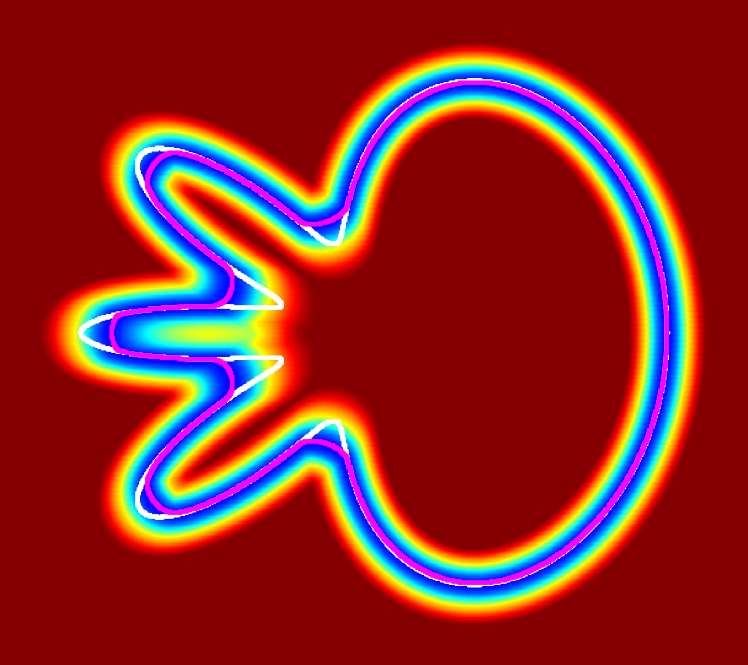
\includegraphics[scale=0.32]{figures/zero-level-set/balance-coefficient-zero-level-set.png}
 \caption{\textbf{Balance coefficient zero level set}. We notice that evolving the initial contour (colored in white) to the zero level set of the balance coefficient (colored in magenta) regularizes the shape with respect to the squared curvature.}
 \label{fig:balance-coefficient-zero-level-set}
 \end{figure}
 
\subsection{Graph cut model}\label{sec:graph-cut-model}

We are going to evolve the initial contour $\partial S$ of some digital shape $S$ to the zero level set of its balance coeficient by computing the minimum cut of some directed graph. Since the balance coefficient is a local quantity, it is sufficient to define the graph in a band around the initial contour.

Let $d_{S}:\Omega \rightarrow \mathbb{R}$ be the signed Euclidean distance transformation with respect to shape $S$. The value $d_{S}(p)$ gives the Euclidean distance between $p \notin S$ and the closest point in $S$. For points $p \in S$, $d_{S}(p)$ gives the negative of the distance between $p$ and the closest point not in $S$.

\begin{definition}{Optimization band}
Let $S \subset \Omega \subset \mathbb{Z}^2$ a digital set and natural number $n>0$. The optimization band $O_n(S)$ is defined as
\begin{align*}
	O_n(S) &:=\left\{ p \in \Omega \; | \; -n \leq d_{S}(p) \leq n \right\}.
\end{align*}
\end{definition}

\begin{definition}{Candidate graph}
Let $S \subset \Omega \subset \mathbb{Z}^2$ a digital set and natural number $n>0$. We define $\mathcal{G}(n,S,\mathcal{V},\mathcal{E})$ as the candidate graph of $S$ with optimization band $n$ such that

\begin{align*}
\mathcal{V} &= \big\{\; v_p \; | \; p \in O_n(S) \;\} \cup \{s,t \big\} \\
\mathcal{E} &= \mathcal{E}_u \cup \mathcal{E}_{st}\\
\mathcal{E}_u &= \big\{ \; \{v_p,v_q\} \; | \; p \in O_n(S) \text{ and } q \in \mathcal{N}_4(p) \; \big\} \\
\mathcal{E}_{st} &= \big\{\; \{s,v_p\} \; | \; d_S(p)=-n \; \big\} \cup \big\{\; \{v_p,t\} \; | \; d_S(p)=n \; \big\}.
\end{align*}

\end{definition}

The vertices $s,t$ are virtual vertices representing the source and target vertices as it is usual in a minimum cut framework. In particular, after the minimum cut is computed, vertices connected to the source will define the new digital shape. The inner (outer) most pixels of the optimization band are connected to the source (target), and we identify such vertices as

\begin{align*}
	\mathcal{V}_s &:=\left\{ v_p \in \Omega \; | \; d_{S}(p) = -n \right\} \\
	\mathcal{V}_t &:=\left\{ v_p \in \Omega \; | \; d_{S}(p) = n \right\}.
\end{align*}

The set $\mathcal{E}_{st}$ comprises all the edges having the source as their starting point or the target as their endpoint. Next, we describe how to set the edges' capacities.

\begin{table}
\begin{center}
\begin{tabular}{|c|c|c|}
\hline
\textbf{edge} $e$ & $\mathbf{c(e)}$ & \textbf{for}\\
\hline
$\{v_p, v_q\}$ & $ u(S,h,r,p) + u(S,h,r,q) $ & $\{v_p,v_q\} \in \mathcal{E}_{u}$\\
\hline
$\{v_p, s\}$ & $M$ & $v_p \in \mathcal{V}_{s}$ \\
\hline
$\{v_p, t\}$ & $M$ & $v_p \in \mathcal{V}_{t}$ \\
\hline
\end{tabular}
\end{center}
,where $M$ is set as twice the highest value of the balance coefficient plus one, i.e.,
%\begin{align*}
%	M &= 1+\max_{p \in O_n(S)} 2*u(S,h,r,p).
%\end{align*}
\begin{align*}
	M &= \max_{e \in \mathcal{E} }{ c(e) }.
\end{align*}
\caption{\textbf{Edge capacity function.}}
\label{tab:edge-capacity}
\end{table}

\subsection{Shape evolution with empty neighborhood of shapes}

In the following, we will refer to the candidate graph of $S$ as $\mathcal{G}(S)$. If necessary, we explicitly define the optimization band value $n$. Starting with digital shape $S^{(t)}$, we construct the candidate graph $\mathcal{G}(S^{(t)})$ and set $S^{(t+1)}$ as the source component of the minimum cut of $\mathcal{G}(S^{(t)})$. We stop the evolution after a given number of iterations.  In figure~\ref{fig:no-neighborhood-shapes-evolution} we show some examples of this process.

\begin{figure}
	\center
	\subfloat[\label{}]{%
	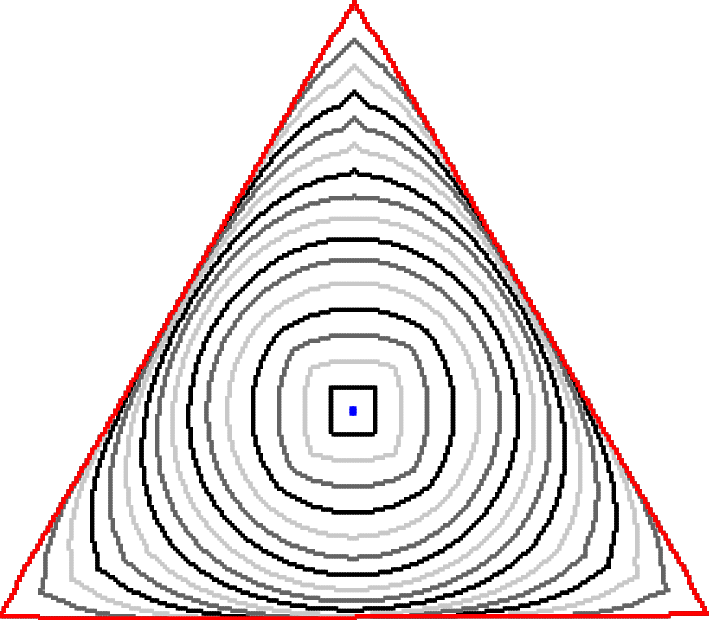
\includegraphics[scale=0.12]{figures/no-neighborhood-flow/triangle.png}}\hspace{2em}%
	\subfloat[\label{}]{%
	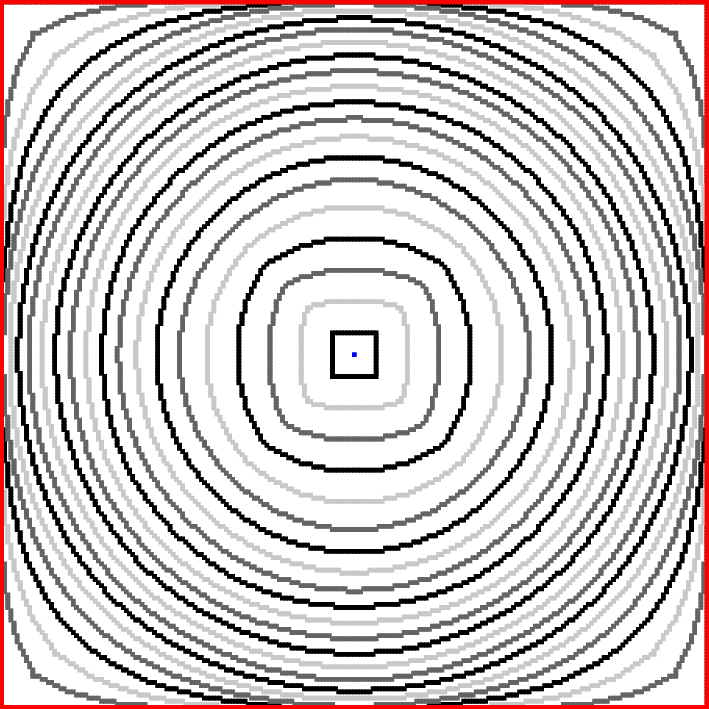
\includegraphics[scale=0.11]{figures/no-neighborhood-flow/square.png}}\hspace{2em}%	
	\subfloat[\label{}]{%
	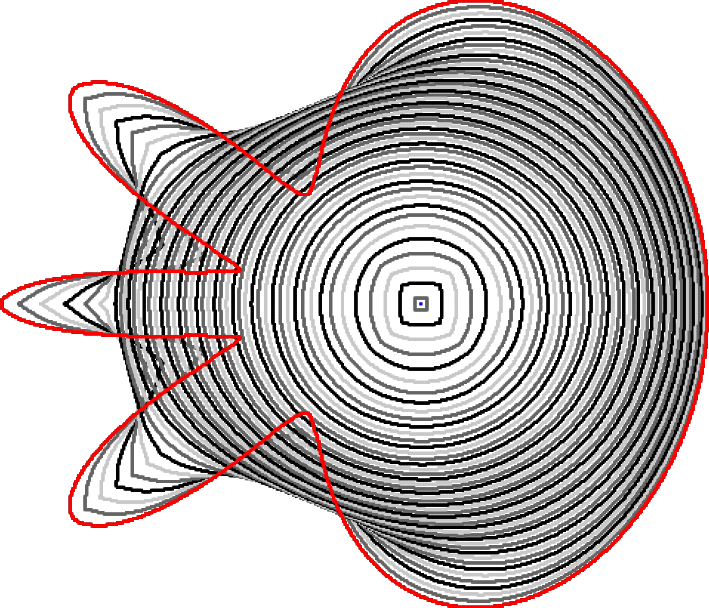
\includegraphics[scale=0.14]{figures/no-neighborhood-flow/flower.png}}	
	\caption{\textbf{No neighborhood of shapes}. Evolution with no neighborhood of shapes defined $(h=1/8,r=2)$. Regions of negative curvature are eliminated and shape tends to converge to a single point. Initial contour is colored in red and each other contour is ploted every 10 iterations.}
	\label{fig:no-neighborhood-shapes-evolution}
\end{figure}

Looking at figure~\ref{fig:no-neighborhood-shapes-evolution}, we may wonder about some properties of this process. For example, a tendance to evolve to convex shapes or shrinking. In fact, we can prove the following

\begin{lemma}[Convexity bias]
\label{claim:convexity-bias} For any initial digital shape $S^{(0)}$, there exists a value $T$ for which $S^{(t)}$ is convex for all $t>T$.
\begin{proof}
The zero level set of $u$ encloses regions of negative curvature. Therefore, such regions vanish away.
\end{proof}
\end{lemma}

\begin{lemma}[Shrinking bias]
\label{claim:shrinking-bias} For all $t$, $Per(S^{(t)}) > Per(S^{(t+1)})$.
\begin{proof}
If $S^{(t)}$ is non-convex, $S^{(t+1)}$ has shorter perimeter by property~\ref{claim:convexity-bias}. If $S^{(t)}$ is convex then curvature is positive everywhere, indicating a shortage of pixels in the balance coefficient. Therefore, the zero level set of balance coeficient is slightly shifted towards the internal part of the shape. The shape shrinks and $Per(S^{(t)}) > Per(S^{(t+1)})$.
\end{proof}
\end{lemma}


These properties are also present in the classical curve shortening flow~\cite{grayson1987heat,ecker2008heat}. This flow is commonly described as the flow that decreases the curve length the quickest. In fact, under the curve shortening flow, one can show that the length varies according to
%
\begin{align*}
\frac{\partial L}{\partial t} = - \int{\kappa ^2 ds}.
\end{align*}
%
The current evolution process does not fulfil the goal of elastica minimization. There is a clear regularization with respect to the squared curvature, but the elastica value eventually increases. We can partially solve this problem by stoping the evolution as soon as the elastica energy increases. However, as shown in figure~\ref{fig:no-neighborhood-shapes-evolution-improve-always}, that may leads to bad local minimum. We can escape local minimum by defining a neighborhood of shapes.

\begin{figure}
	\center
	\subfloat[\label{}]{%
	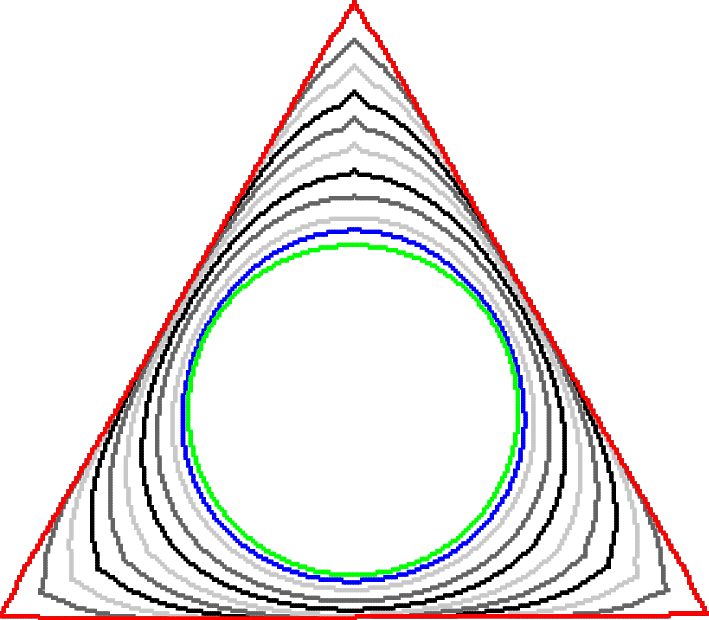
\includegraphics[scale=0.12]{figures/no-neighborhood-flow-improve-always/triangle.png}}\hspace{2em}%
	\subfloat[\label{}]{%
	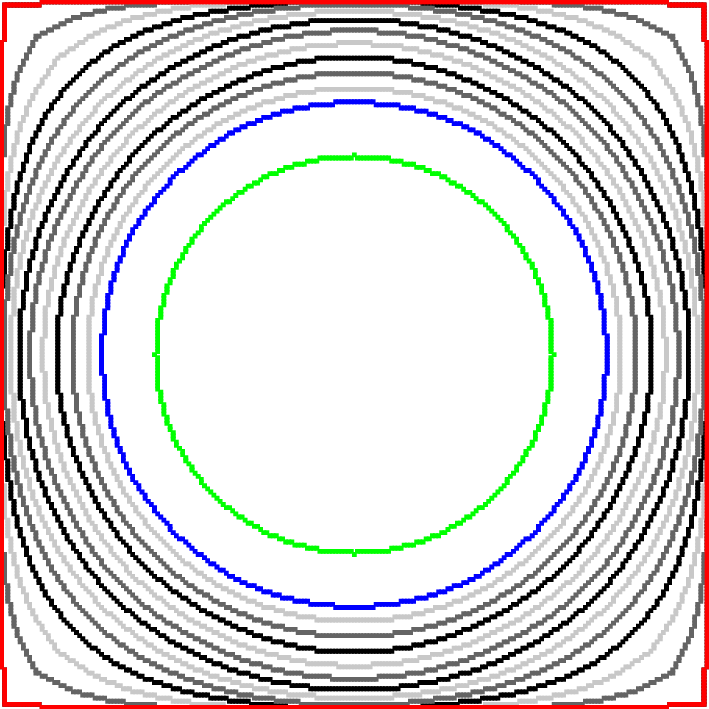
\includegraphics[scale=0.11]{figures/no-neighborhood-flow-improve-always/square.png}}\hspace{2em}%	
	\subfloat[\label{}]{%
	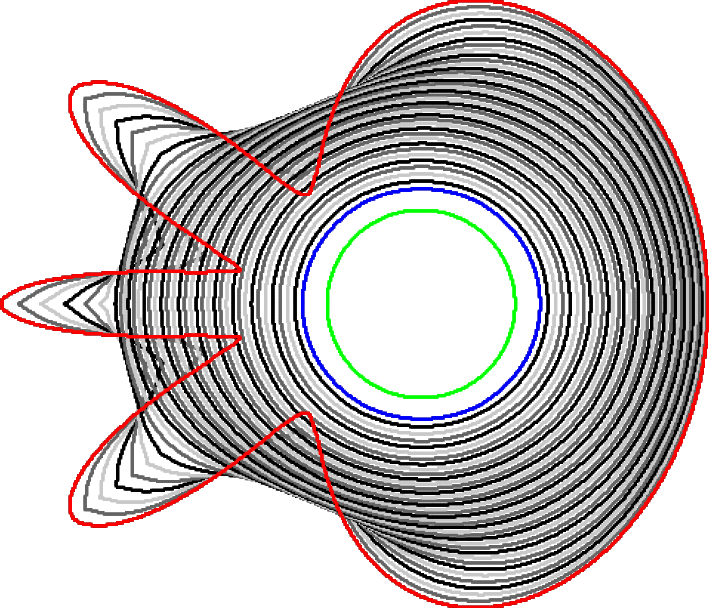
\includegraphics[scale=0.14]{figures/no-neighborhood-flow-improve-always/flower.png}}	
	\caption{\textbf{Stop if elastica increases}. In red the initial contour and in blue the final contour given by the evolution process with no neighborhood of shapes $\vec{\Theta} = (h=1/8,r=2,\alpha=1/64,\beta=1)$. The optimum contour is highlighted in green (a disk of radius $8$). Intermediate contours are ploted every 10 iterations.}
	\label{fig:no-neighborhood-shapes-evolution-improve-always}
\end{figure}

\subsection{Neighborhood of shapes}

The model as stated is incapable to find global optimal solutions. Consider the following example: we start with a disk of radius $8$ and we want to minimize it with respect the elastica with $\alpha =1/256, \beta=1$. The optimum shape is the disk of radius $16$. However, by lemmas~\ref{claim:convexity-bias} and~\ref{claim:shrinking-bias}, the shape will never evolve to a disk of higher radius.

Fortunately, we can fix this problem by defining a neighborhood of shapes. 

\begin{definition}[Neighborhood of shapes]
	Let $S$ a digital shape. We define its neighborhood $\mathcal{N}(S)$ as the set
	\begin{align*}
		\mathcal{N}(S) &= S \cup S^{+1} \cup S^{-1},
	\end{align*}
	where $S^{+1}$ ($S^{-1}$) denotes a morphologic dilation (erosion) by a square of side $1$.
\end{definition}

Instead of setting $S^{(t+1)}$ as the source component of the minimum cut of $G(S^{(t)})$, we construct a collection of candidate graphs, one for each member of $\mathcal{N}(S^{(y)}$. Then, we compute the minimum cut and evaluate the elastica energy in the resulting digital set. Finally, we pick the one with lowest energy. The GraphFlow (GF) model~\ref{alg:graphflow-algorithm} summarizes the process and figure~\ref{fig:graph-flow-experiments} include some experiments.

\begin{algorithm}
 \SetKwData{It}{k}
 \SetKwData{MIt}{maxIt}
 \SetKwData{Delta}{delta}
 \SetKwInOut{Input}{input}\SetKwInOut{Output}{output}
 \SetKwComment{comment}{//}{}
 
 \Input{A digital set $S$; the optimization band $n$; parameter vector $\vec{\theta}=(h,r,\alpha,\beta)$; the maximum number of iterations \MIt;} 
 \BlankLine
 $S^{(0)} \longleftarrow S$\; 
 \BlankLine
 $k \longleftarrow 0$\;
 \While{ \It $<$ \MIt  }{ 	
	\comment{Candidate selection} 
	$\mathcal{C}^{(k)} \longleftarrow \bigcup_{S' \in \mathcal{N}(S^{(k)})} \Big\{ D(Q) \; | \; mincut(Q,\mathcal{G}(S') \Big\}$ \;

	\BlankLine
	\comment{Candidate validation}
	$S^{(k+1)} \longleftarrow \displaystyle \argmin_{ S' \in \mathcal{C}^{(k)} }{ \hat{E}_{\vec{\theta}}(S')}$\; 	
	\It $\longleftarrow$ \It $+1$\;
	
 }
 \caption{GraphFlow algorithm.}
 \label{alg:graphflow-algorithm}  
\end{algorithm}

\begin{figure}
\begin{minipage}{0.25\textwidth}
\center
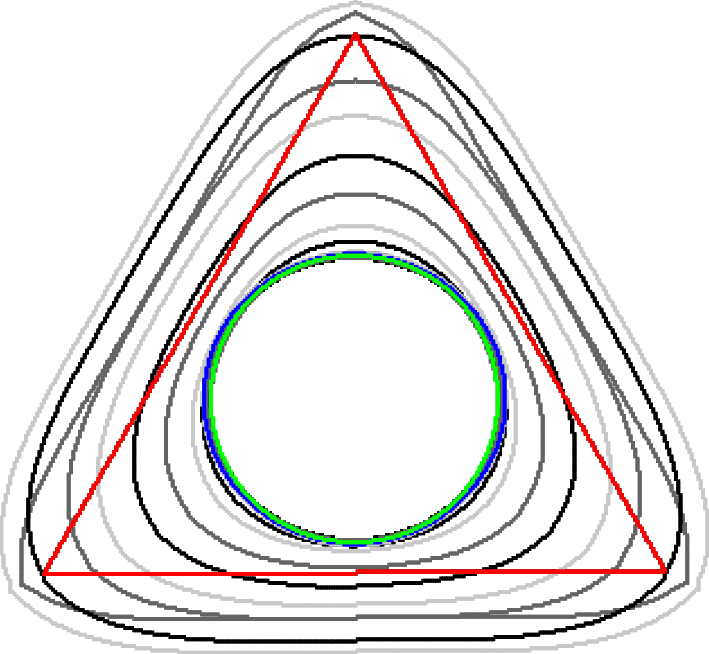
\includegraphics[scale=0.10]{figures/shape-flow/summaries-r8/triangle.png}

\vspace{1.5em}

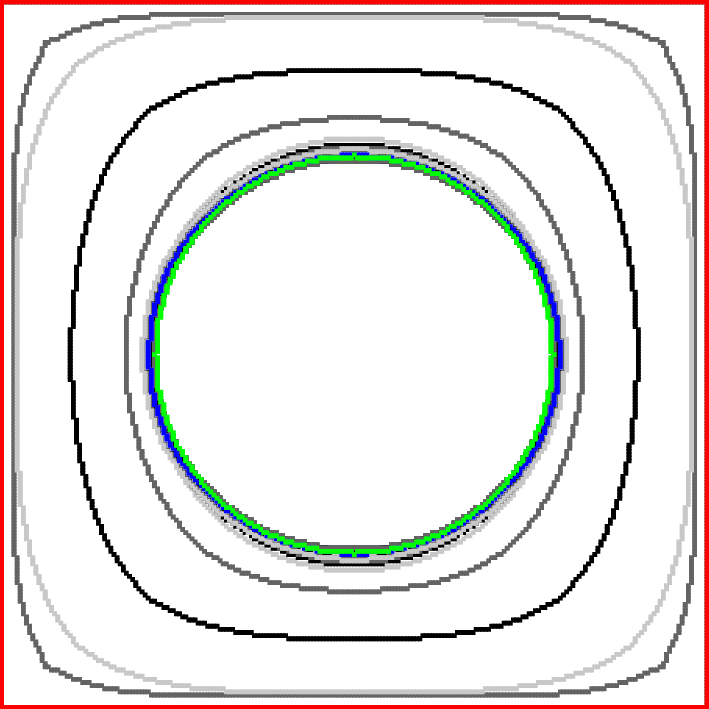
\includegraphics[scale=0.08]{figures/shape-flow/summaries-r8/square.png}

\vspace{1.5em}

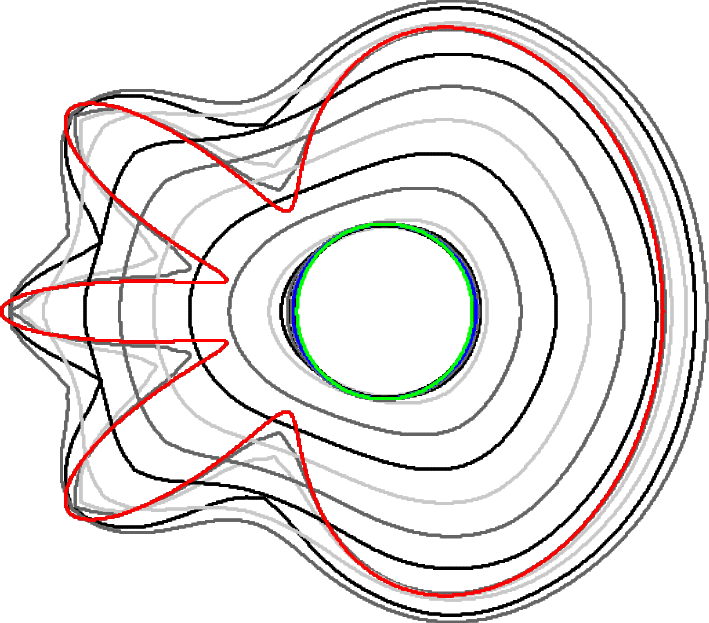
\includegraphics[scale=0.10]{figures/shape-flow/summaries-r8/flower.png}

\vspace{1.5em}

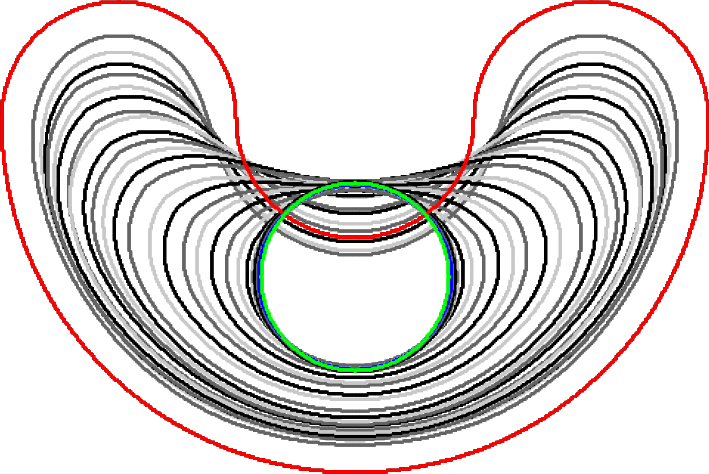
\includegraphics[scale=0.10]{figures/shape-flow/summaries-r8/bean.png}
\end{minipage}%
\begin{minipage}{0.75\textwidth}
\center
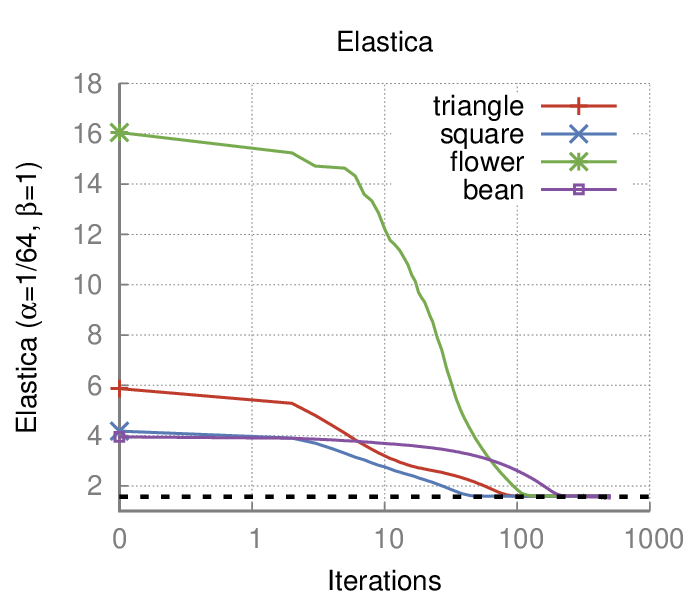
\includegraphics[scale=0.22]{figures/shape-flow/plots/elastica.png}

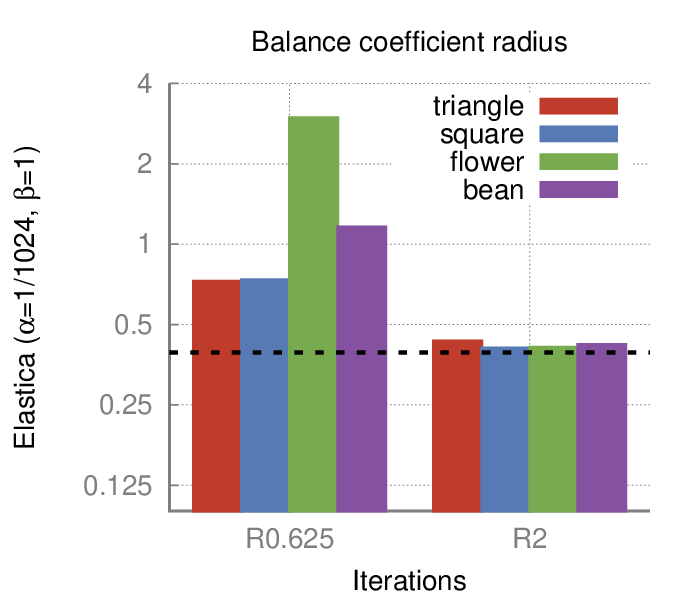
\includegraphics[scale=0.22]{figures/shape-flow/plots/bars.png}
\end{minipage}
\caption{\textbf{GraphFlow experiments}. In the left, the evolution of various shapes given by the GraphFlow model $(h=1/8,r=2)$. The red and blue contours highlight initial and final contour. The green contour is the optimum solution. The top right graph describes the reduction in elastica energy. The dotted line marks the optimum energy value (a disk of radius $8$). The bottom right graph points out the importance of a right choice of the balance coefficient radius (the optimum solution in this case is a disk of radius 32).}
\label{fig:graph-flow-experiments}
\end{figure}

Remarkably, the GF model escapes premature local minimum and even achieves the global optimum of the elastica energy for some cases. Moreover, due to the neighborhood of shapes, the GF model can also expand. In figure~\ref{fig:graph-flow-expand} we show the results of elastica minimization for $\vec{\Theta} = ( r=2,h=1/8,\alpha=1/1024,\beta=1 )$. The GF model correctly expands the shapes to the optimum disk of radius $32$. However, we may have a premature interruption of the evolution if a small balance coefficient radius is chosen, as illustrated in the bottom right graph of figure~\ref{fig:graph-flow-experiments}.

\begin{figure}
\center
\subfloat[]{
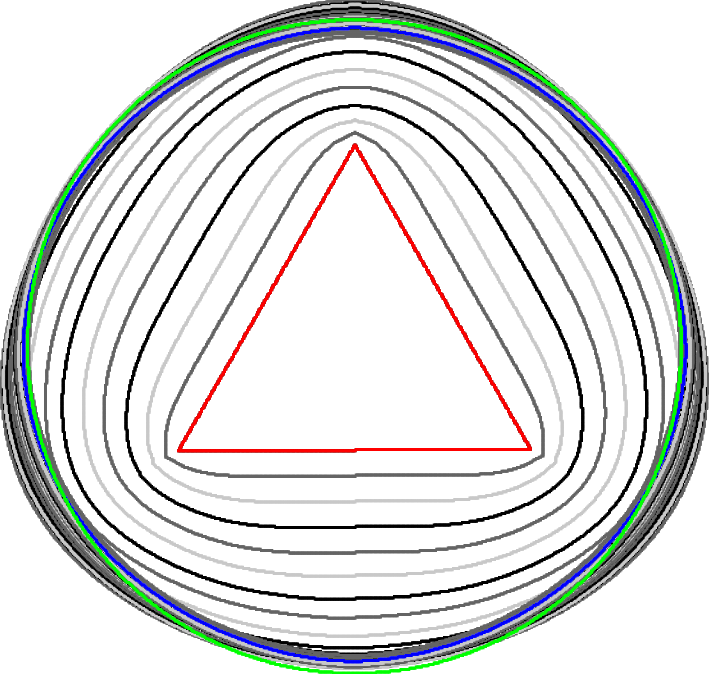
\includegraphics[scale=0.13]{figures/shape-flow/summaries-r32/triangle.png}}\hspace{1.5em}%
\subfloat[]{
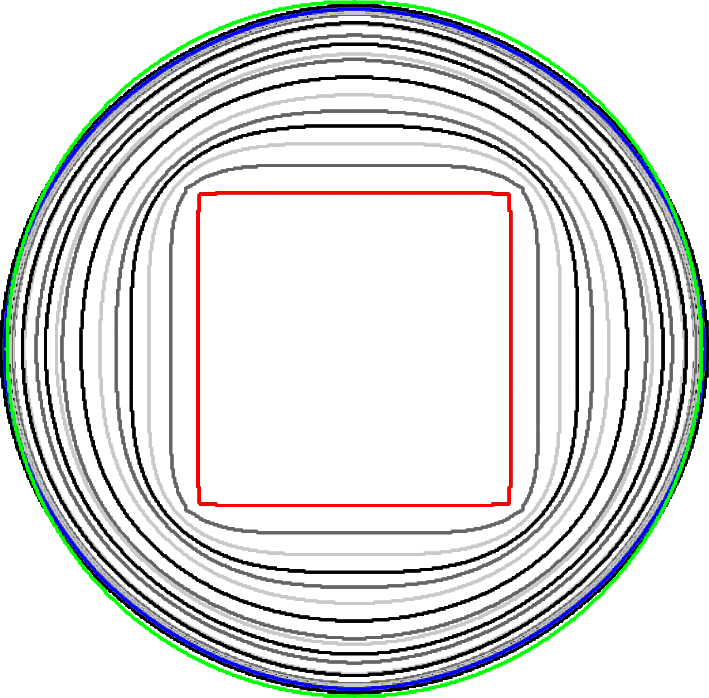
\includegraphics[scale=0.13]{figures/shape-flow/summaries-r32/square.png}}\hspace{1.5em}%
\subfloat[]{
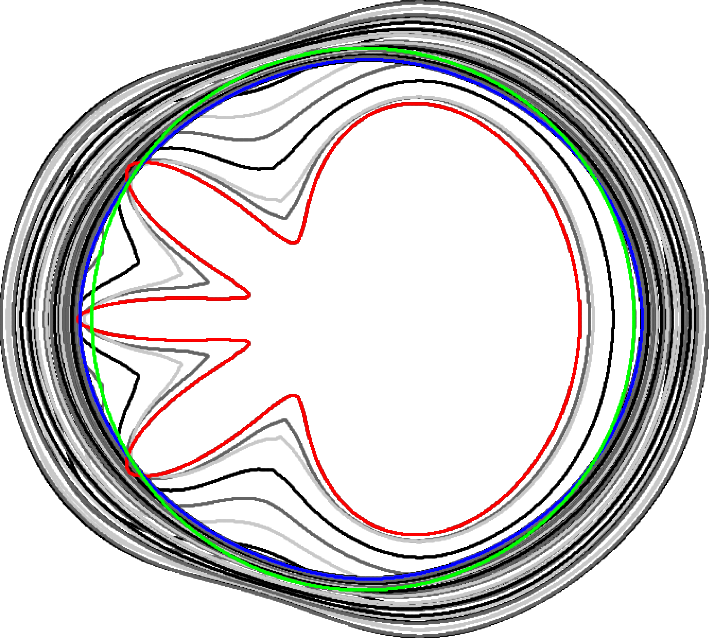
\includegraphics[scale=0.15]{figures/shape-flow/summaries-r32/flower.png}}
\caption{\textbf{GF model can expand}. Shapes evolutions given by GF model with $\vec{\Theta}(h=1/8,r=2,\alpha=1/1024, \beta=1)$ as the digital elastica parameters. The green contour highlights the optimum shape (a disk of radius $32$).}
\label{fig:graph-flow-expand}
\end{figure}

The GF model with neighborhood of shapes is faster. The lower density of plotted curves in figure~\ref{fig:graph-flow-experiments} compared with those of figure~\ref{fig:no-neighborhood-shapes-evolution-improve-always} indicates that the speed of convergence to global optimum is increased when a neighborhood of shapes is used. Moreover,  all the steps of the GF model, except the min-cut computation, can be executed in parallel. Table~\ref{tab:summary-graph-flow-running-time} shows the running times where the candidate graphs are evaluated in parallel. These times can be further improved by making parallel the computation of the balance coefficient and also the digital elastica evaluation.

\begin{figure}[h!]
\center
\captionsetup{type=table}
\footnotesize
\begin{tabular}{|l|c|c|c|c|}
\hline
& Pixels & It & Time & Time/It\\
\hline
Triangle & 33256 & 100 & 15s & 0.3s \\
Square & 51259 & 50 & 31s & 0.3s \\
Flower & 119789 & 150 & 78s & 0.5s \\
\hline
\end{tabular}
\caption{\textbf{Running time of GF algorithm}. The GF algorithm achieves running times lower than one second per iteration when the shape neighbors are evaluated separately. The algorithm is completly parallelizable and these running times can be further improved.}
\label{tab:summary-graph-flow-running-time} 
\end{figure}

Finnaly, the GF algorithm is easily modifiable to accomodate image terms, which makes it suitable for image processing tasks. Next, we are going to explore some of these possibilitites in image segmentation.

\section{Applications in image processing}

The GF model can be extended to include a data fidelity term. In this section we explore the potential of the GF model to be used in image processing tasks. We present the results of two experiments. The first is targeted to supervised segmentation and the second to unsupervised segmentation. Since we do not have an explicit expression for the input shapes (that is, the objects to segment), the grid resolution is set to $h=1$ in all experiments. The experiments were executed in [machine configuration].


\subsection{Supervised segmentation}

The goal of this experiment is to illustrate the regularization properties of the GF model and to highlight the role of the data term in our approach. The data term employed in this experiment is the same used by Boykov-Jolly classical graph cut model~\cite{boykov01graphcut}. 

\subsubsection{Data term}
We are going to update the graph construction described in section~\ref{sec:graph-cut-model} to accomodate the data term. In particular, we define two new sets of vertices $\mathcal{V}_{fg}$ and $\mathcal{V}_{bg}$ as the set of foreground and background seeds, respectively. Those are given as input.

Let $\vec{x} \in \{0,1\}^{|S|}$ represent the label of each pixel in the image ($0$ for background and $1$ for foreground). We define the data term as
%
\begin{align*}
	data(S) &= \gamma_r \sum_{p \in S}{ \psi(x_p) } + \gamma_b \sum_{p \in S}\sum_{q \in \mathcal{N}_{4}(p)}{\psi_{(p,q)}},
\end{align*}
where $\gamma_r \geq 0$ and $\gamma_b \geq 0$ are parameters controlling the influence of the regional and boundary terms, respectively. Given the image $I:\Omega \rightarrow [0,1]^3$, the unary and pairwise terms are defined as
\begin{align*}
	\psi(x_p) &= \left\{ \begin{array}{ll}
	-\ln  H_{bg}\big( I(p) \big), & \text{if } x_p=0  \\[1em]	
	-\ln  H_{fg}\big( I(p) \big), & \text{if } x_p=1,
	\end{array}\right.\\[1em]
	\psi_{(p,q)} &= \left\{ \begin{array}{ll}
	\displaystyle \exp{ \left(- \frac{1}{ |(p,q)| }\frac{(I(p) - I(q))^2}{2\sigma^2} \right) }, & q \in \mathcal{N}_4(p) \\[1em]
	0, & \text{otherwise}.
	\end{array}\right.
\end{align*}
%
The terms $H_{bg}$ and $H_{fg}$ are mixed Gaussian distribution constructed from the foreground and background seeds. The updated capacity function is described in table~\ref{tab:updated-capacity-function}.
%
\begin{table}
\setlength{\extrarowheight}{0.75em}
\begin{center}
\begin{tabular}{|c|c|c|}
\hline
\textbf{edge} $e$ & $\mathbf{c(e)}$ & \textbf{for}\\
\hline
$\{v_p, v_q\}$ & $\beta \cdot \big(u(S,h,r,p) + u(S,h,r,q)\big) + \gamma_b \cdot \psi_{(p,q)}$ & $\{v_p,v_q\} \in \mathcal{E}_{u}$\\
\hline
\multirow{3}{*}{$\{v_p, s\}$} & $\gamma_r \cdot \psi(0)$ & $p \in O_n(S), v_p \notin \mathcal{V}_{fg} \cup \mathcal{V}_{bg}$\\
& $M$ & $v_p \in \mathcal{V}_{s} \cup \mathcal{V}_{fg}$ \\
\hline
\multirow{3}{*}{$\{v_p, t\}$} & $\gamma_r \cdot \psi(1)$ & $p \in O_n(S), v_p \notin \mathcal{V}_{fg} \cup \mathcal{V}_{bg}$ \\
& $M$ & $v_p \in \mathcal{V}_{t} \cup \mathcal{V}_{bg}$  \\
\hline
\end{tabular}
\end{center}
where the constant $M$ is defined such that
\begin{align*}
M &= \max_{e \in \mathcal{E} }{ c(e) }.
\end{align*}
\caption{\textbf{Updated capacities.} The capacity function of table~\ref{tab:capacity-function} is updated to accommodate the data term.}
\label{tab:updated-capacity-function}
\end{table}
%
%
To handle bias due to magnitude difference between the terms, we normalize them in groups. Boundary and regional capacities are normalized to the interval $[0,1]$ with respect their values. The same is done, separately, for the curvature term.

To minimize parameter dependence from the image input, we also execute parameter normalization. Given parameters $\alpha, \gamma_b, \gamma_r$ and an initial segmentation $I_0$, we apply the following normalization factors.
%
\begin{align*}
	\alpha & = \alpha \times 4\pi^2/Per^2 \\
	\gamma_r & = \gamma_r \times \hat{E}(I_0)/Data(I_0) \\	
	\gamma_b & = \gamma_b \times \hat{E}(I_0)/Data(I_0)		
\end{align*}
%
%
\subsubsection{Experiment}
We need an initial contour to start the GF model. The initial contour is given by the grabcut algorithm ~\cite{rother04grabcut}, a variant of classical graph cut segmentation~\cite{boykov01graphcut} which is implemented in the OpenCV library.

For this experiment we used a selection of $100$ images of the Validation 2017 subset of the Coco dataset~\cite{lin2014microsoft}. The Coco dataset comprises over $328$k images spreaded over $91$ categories and $11$ super-categories. Table~\ref{tab:image-categories-distribution} summarizes the selected images by super-category. 
%
%
\begin{table}
\begin{tabular}{cccccc}
\hline
\textbf{Person} & \textbf{Vehicle} & \textbf{Food} & \textbf{Animal} & \textbf{Outdoor Obj.} & \textbf{Sports} \\
\hline
24 & 22 & 9 & 34 & 2 & 1 \\
\hline
\textbf{Kitchenware} & \textbf{Furniture} & \textbf{Appliance} & \textbf{Electronics} & \textbf{Indoor Obj.} & \\
\hline
2 & 1 & 0 & 1 & 5 & \\
\hline
\end{tabular}
\caption{\textbf{Images distribution.} The amount of selected images per Coco super-category.}
\label{tab:image-categories-distribution}
\end{table}
%
%

This experiment consisted in manually select foreground and background seeds for each selected image; compute the grabcut segmentation; and then use the grabcut segmentation as input for two versions of the GF model: one with the data term described in the previous section and another without. In figure~\ref{fig:coco-experiment-sample} we show a sample of the images used in the experiment. All the results are available online and can be conveniently visualized in this webpage. 

In table~\ref{tab:coco-experiment-parameter} we list the GF parameters for this experiment.

\begin{table}
\center
\begin{tabular}{cccc}
\textbf{Estimation radius} & \textbf{Opt. band width} & \textbf{Neighborhood size} & \textbf{Iterations} \\
5 & 4 & 3 & 20\\
\hline
$\boldsymbol{\alpha}$ & $\boldsymbol{\beta}$ & $\boldsymbol{\gamma_b}$ & $\boldsymbol{\gamma_r}$\\
10 & 1 & 1 & 1 \\
\hline
\end{tabular}
\caption{\textbf{Supervised experiment parameters}. The list of the GF model parameters for the supervised segmentation experiment.}
\label{tab:coco-experiment-parameter}
\end{table}
%
%
%
%
\begin{figure}
\center
\subfloat[Coco annotations for kite, moto and giraffe]{
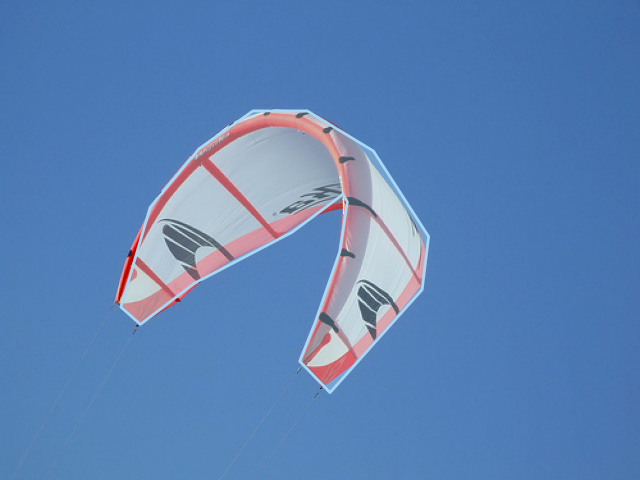
\includegraphics[scale=0.2]{figures/coco/kite/coco-annotation.png}\hspace{1em}
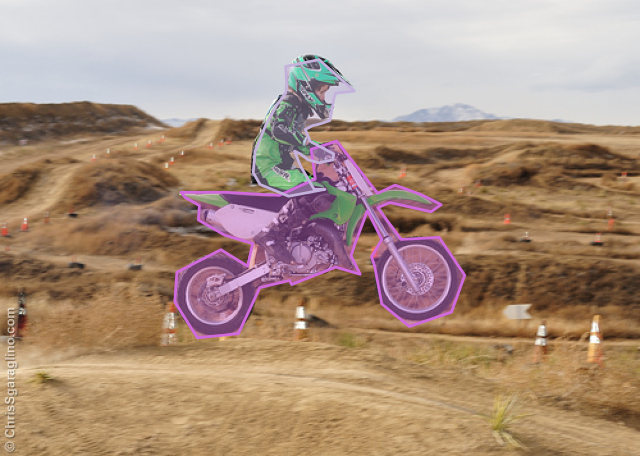
\includegraphics[scale=0.2]{figures/coco/moto/coco-annotation.png}
\hspace{1em}
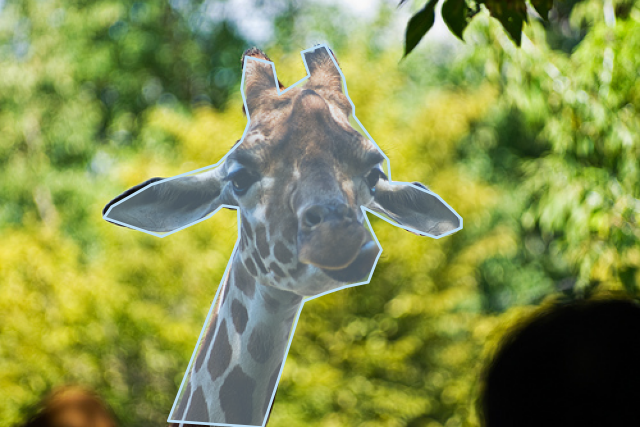
\includegraphics[scale=0.2]{figures/coco/giraffe/coco-annotation.png}
}%

\subfloat[Graph cut segmentation]{
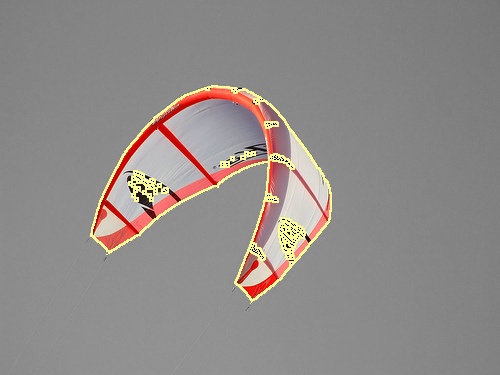
\includegraphics[scale=0.2]{figures/coco/kite/gc-seg.png}
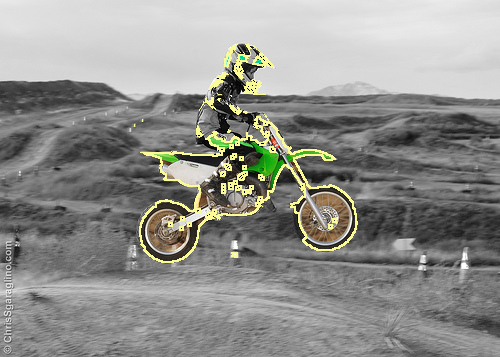
\includegraphics[scale=0.2]{figures/coco/moto/gc-seg.png}
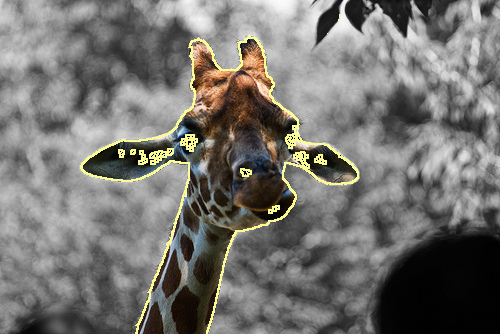
\includegraphics[scale=0.2]{figures/coco/giraffe/gc-seg.png}
}

\subfloat[GF correction with data term]{
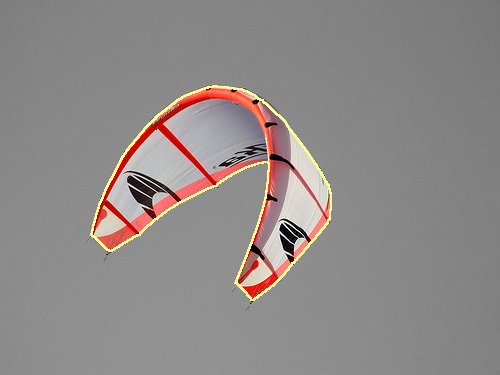
\includegraphics[scale=0.2]{figures/coco/kite/corrected-seg-with-data.png}
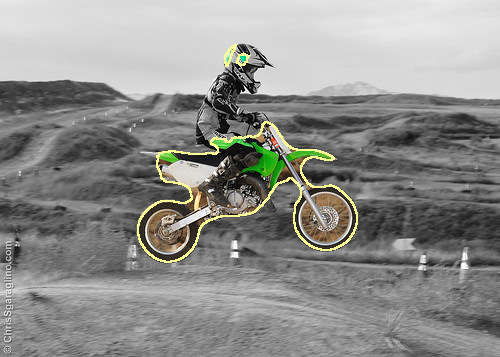
\includegraphics[scale=0.2]{figures/coco/moto/corrected-seg-with-data.png}
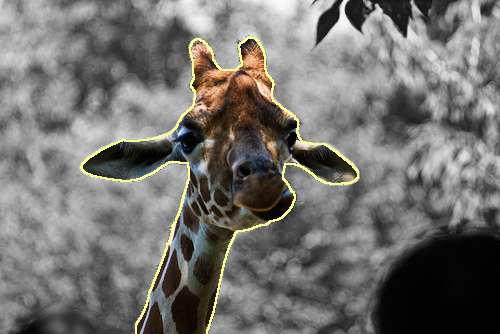
\includegraphics[scale=0.2]{figures/coco/giraffe/corrected-seg-with-data.png}
}

\subfloat[GF correction without data term]{
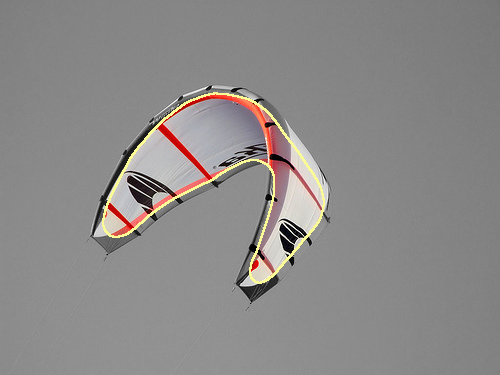
\includegraphics[scale=0.2]{figures/coco/kite/corrected-seg-without-data.png}
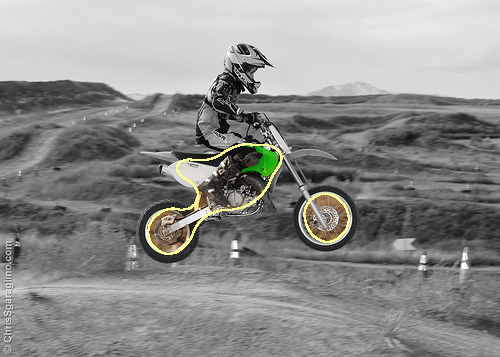
\includegraphics[scale=0.2]{figures/coco/moto/corrected-seg-without-data.png}
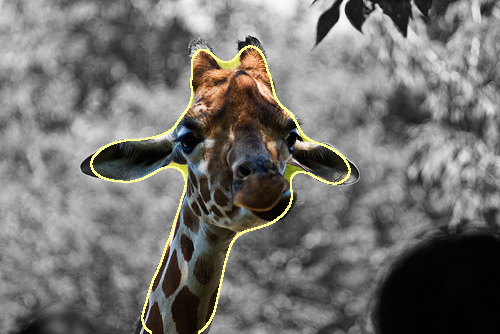
\includegraphics[scale=0.2]{figures/coco/giraffe/corrected-seg-without-data.png}
}
\caption{\textbf{Results sample of the supervised segmentation experiment}. Coco annotations are shown in the first line. In the next rows we present the same image segmented by grabcut and corrected by the GF model with and without data term.  }
\label{fig:coco-experiment-sample}
\end{figure}
%
%
%
The first observation is that the GF model regularizes the initial grabcut segmentation contour with respect to the elastica energy. That is illustrated in figure~\ref{fig:coco-tangent-profile} in which we display the tangent profile of the grabcut segmentation and the one corrected by the GF model. The value of the elastica energy of the contour and its number of inflection points is also greatly reduced, as it is summarized in figure~\ref{fig:coco-summary-regularization}.

The second observation is that the data term has an important role in the quality of the segmentation with respect to precision and recall metrics, as shown in the box plot of figure~\ref{fig:coco-summary-precision-recall}. That means that by using a model with no data term, such as threshold dynamics, is not sufficient to recover segmentations of good quality. In fact, executing the GF model without data term will eventually transform the contour in one or more circles, and we can have an arbitrary bad value for the recall. We can see some of these undesirable effects in the fourth line of figure~\ref{fig:coco-experiment-sample}: the kite area is over reduced; the motorcycle is separated in two disconnected components; and the giraffe loses part of its ears.

The third observation is that the GF model presents the completion effect that is expected from regularization by elastica energy. That property is particularly useful for the segmentation of thin and elongated objects, but not only. It also helps to remove oversegmented components which are particularly common in graph cut based models. In figure~\ref{fig:coco-completion} we give some examples of contour completion.

Finally, we remark that all images were executed using the same set of parameters. That is not ideal. Low resolution images should be segmented using a smaller estimation radius, for example. Therefore, all the results presented here could be eventually improved by tunning the parameters accordingly. An example of this is given in figure~\ref{fig:coco-parameter-tuning}.

%
%
%
%
\begin{figure}
\center
\subfloat[Grabcut segmentation (left) and corrected segmentation by GF (right).]{
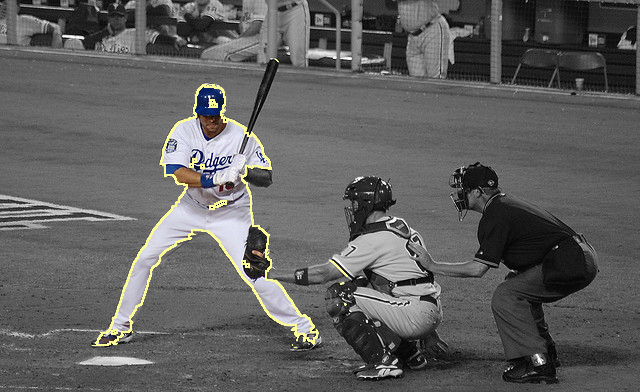
\includegraphics[scale=0.25]{figures/coco/baseball/gc-seg.png}\hspace{1em}
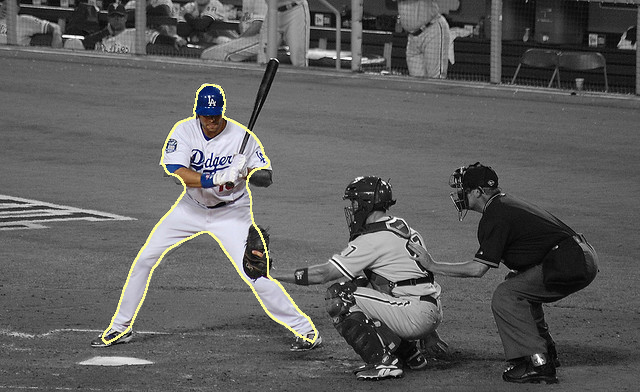
\includegraphics[scale=0.25]{figures/coco/baseball/corrected-seg-with-data.png}
}

\subfloat[Tangent profile for grabcut (left) and GF corrected (right) segmentations.]{
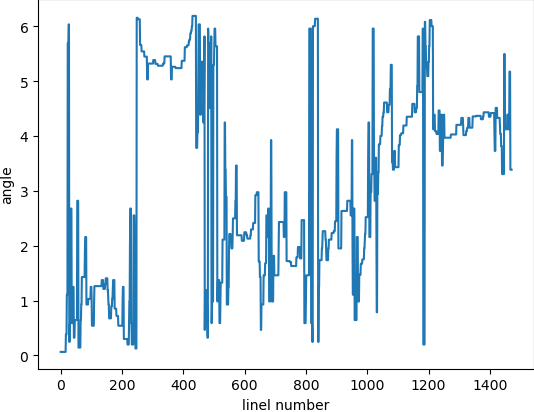
\includegraphics[scale=0.42]{figures/coco/baseball/tangent-profile-gc.png}\hspace{1em}
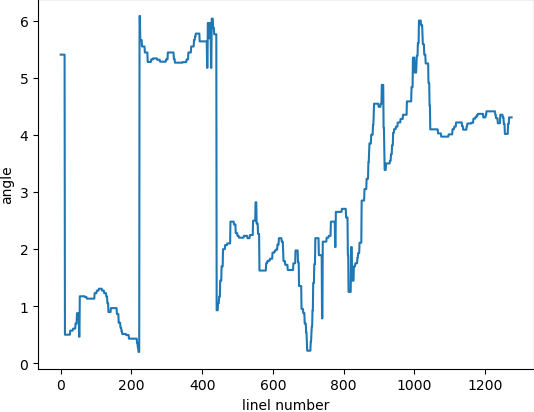
\includegraphics[scale=0.42]{figures/coco/baseball/tangent-profile-cc.png}
}
\caption{\textbf{Contour regularization.} The GF model normlalizes the contour with respect the elastica energy. This is illustrated by the tangent profile of the grabcut segmentation and the one corrected by GF.}
\label{fig:coco-tangent-profile}
\end{figure}
%
%
\begin{figure}
\center
\subfloat[Recall and precision results with respect to Coco annotations.\label{fig:coco-summary-precision-recall} ]{
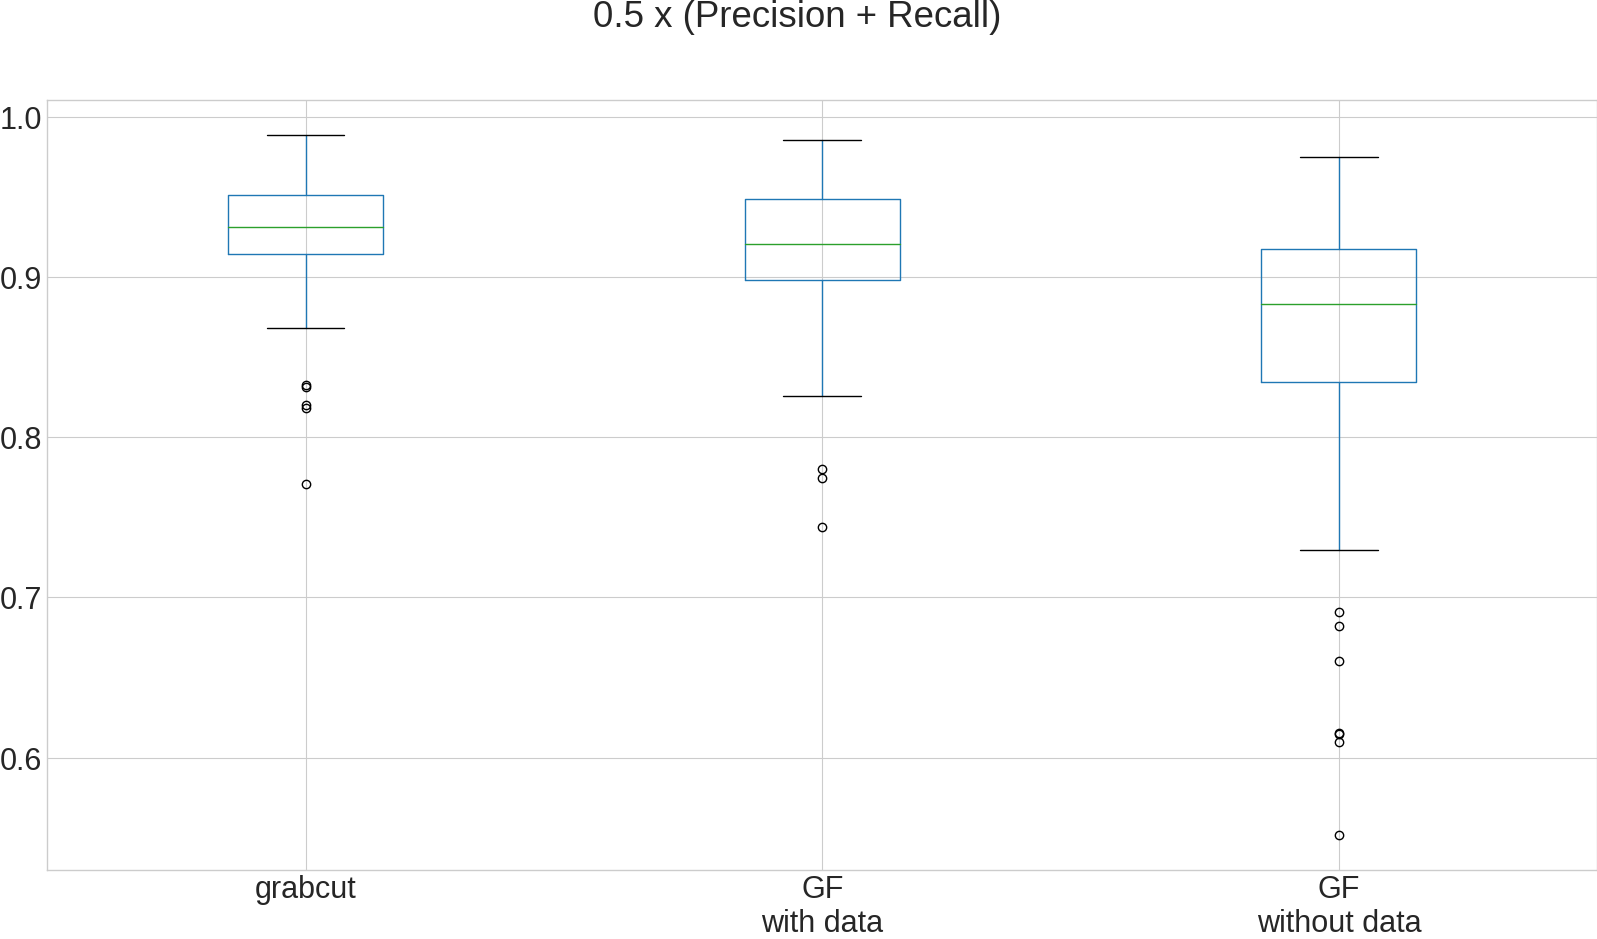
\includegraphics[scale=0.25]{figures/coco/box-plot-mixed.png}
}

\subfloat[Contour regularization metrics for GF with respect grabcut.\label{fig:coco-summary-regularization}]{
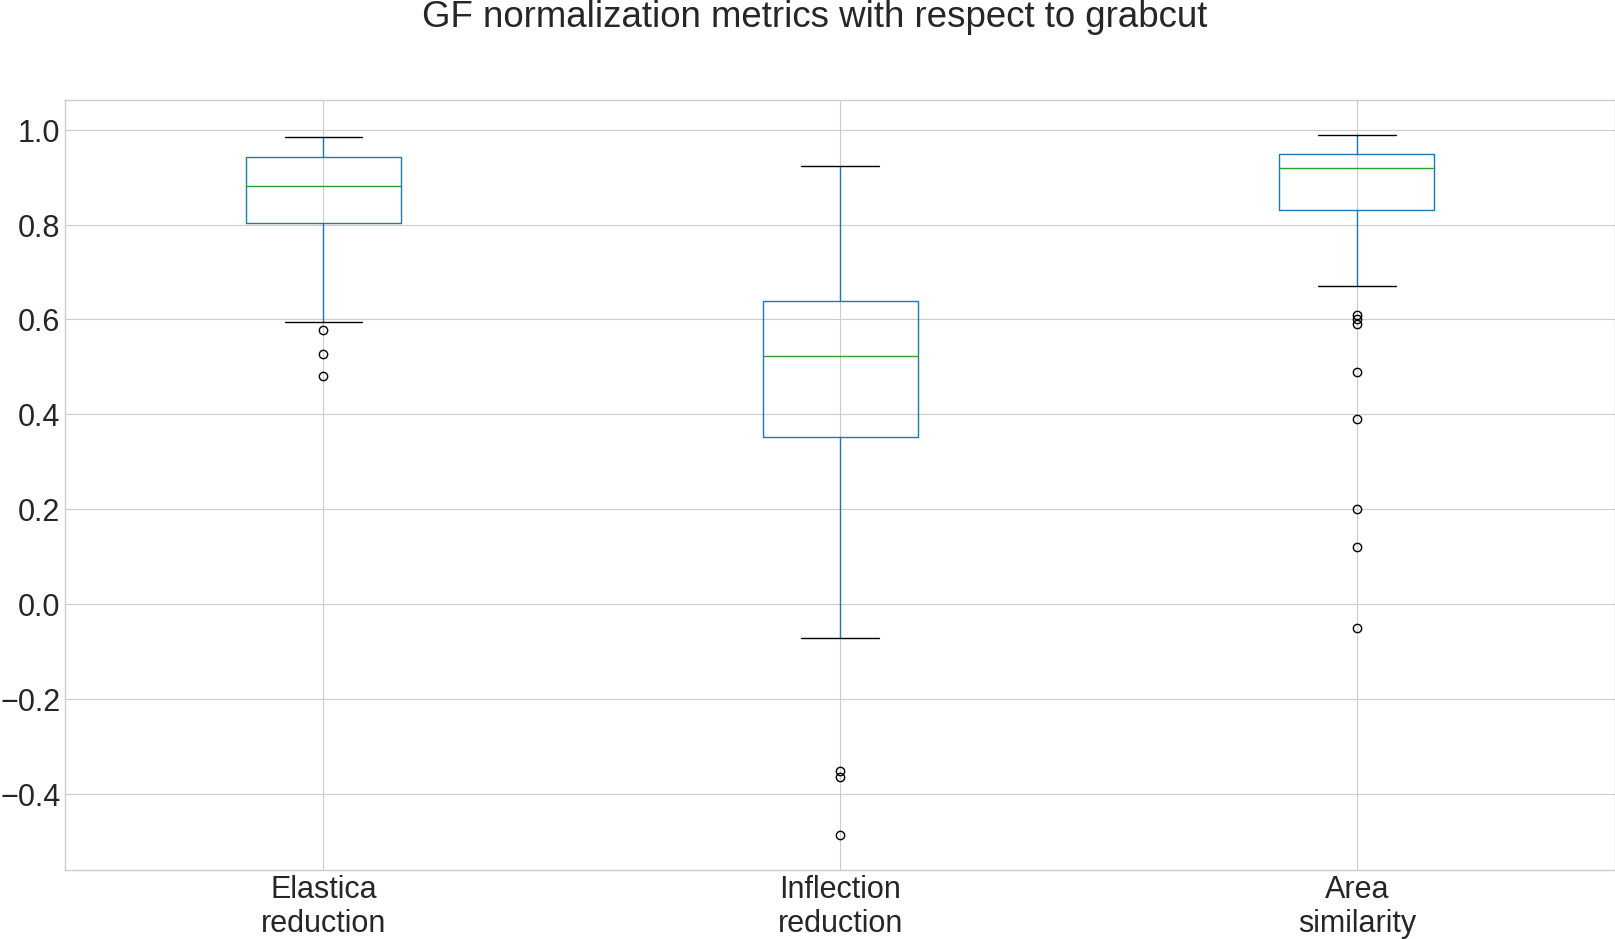
\includegraphics[scale=0.25]{figures/coco/box-plot-correction.png}
}

\caption{\textbf{Summary statistics.} The GF model give results as good as grabcut with respect to precision and recall, but with a much simpler and easy to describe (and store) contour.}
\end{figure}
%
%
\begin{figure}
\center
\subfloat[Using $r=5$ (mm=$0.78$)]{
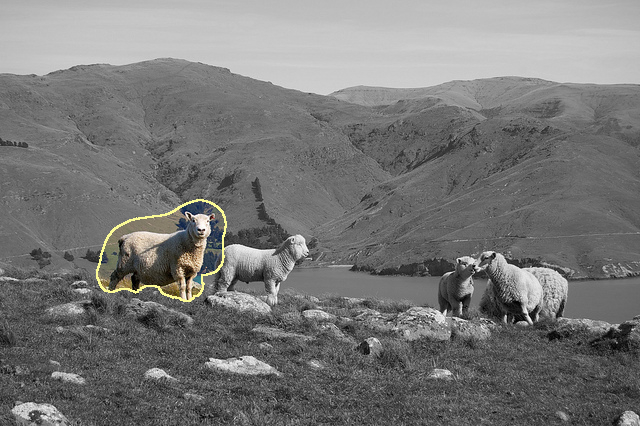
\includegraphics[scale=0.25]{figures/coco/parameter-tuning/corrected-seg-with-data-r5.png}}\hspace{1em}
\subfloat[Using $r=3$ (mm=$0.94$)]{
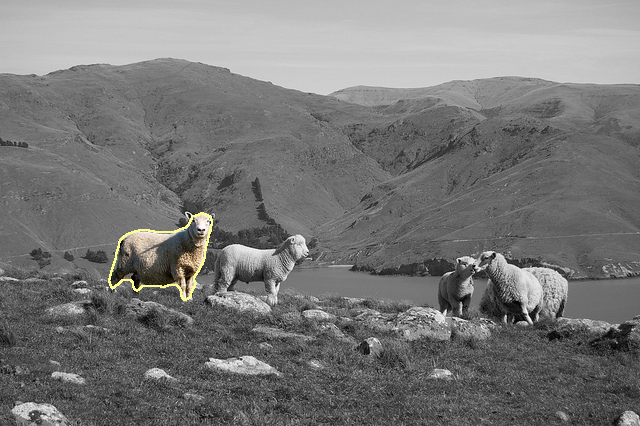
\includegraphics[scale=0.25]{figures/coco/parameter-tuning/corrected-seg-with-data-r3.png}}
\caption{\textbf{Parameter tuning.} The GF model was executed with the same set of parameters for all images, but we can recover better results by tuning the parameter for each image. In this example, the low scale of the image asks for a lower estimation radius. The mixed metric goes from $0.78$ to $0.94$. }
\label{fig:coco-parameter-tuning}
\end{figure}
%
%
\subsection{Unsupervised binary segmentation}
The goal of this experiment is to illustrate the flexibility of the GF model with respect to the data fidelity term. In this experiment, we employed a Chan-Vese allike data term~\cite{chan01}, i.e., we penalize the square mean error between pixel intensity and the average foreground color (similarly for the background). We define the initial solution as an uniform collection of disks covering the image domain.

In this application, our strategy to avoid local minima is slightly different. We use a larger random neighborhood of shapes and we allow evolution if and only if the previous energy value is reduced. This strategy lead to higher running times, but since the digital components are treated independently, we believe that running times can be vastly reduced by implementing a more agressive parallelization, for example, using GPUs. 

The algorithm can evolve the contours to favor its completion or its breaking according to the relative weights given for the elastica and data terms. We show the results of some experiments in figure~\ref{fig:GF-chan-vese-alike}.

\begin{figure}
\center
\subfloat[Segmentation by grabcut]{
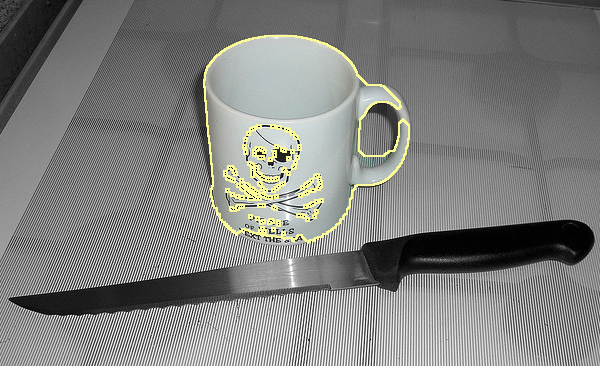
\includegraphics[scale=0.185]{figures/coco/completion/cup/gc-seg.png}\hspace{0.5em}
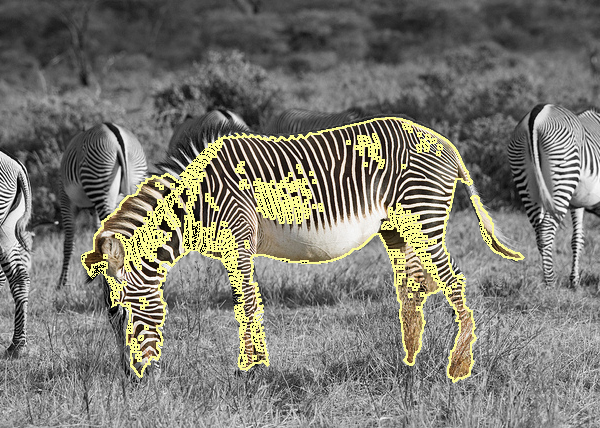
\includegraphics[scale=0.16]{figures/coco/completion/zebra/gc-seg.png}
\hspace{0.5em}
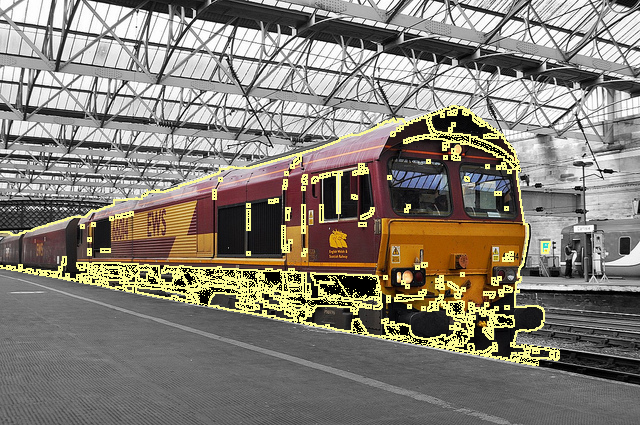
\includegraphics[scale=0.16]{figures/coco/completion/train/gc-seg.png}
}%

\subfloat[Segmentation corrected by GF]{
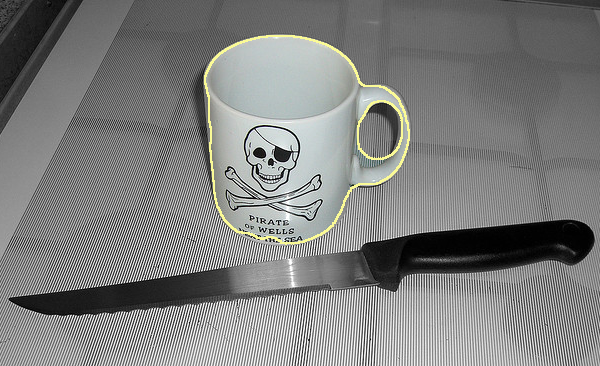
\includegraphics[scale=0.185]{figures/coco/completion/cup/corrected-seg-with-data.png}\hspace{0.5em}
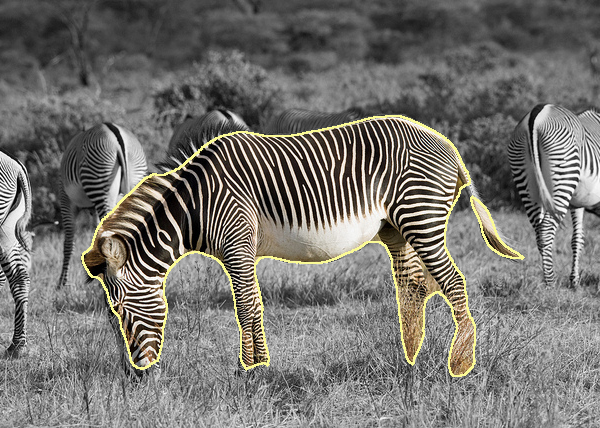
\includegraphics[scale=0.16]{figures/coco/completion/zebra/corrected-seg-with-data.png}
\hspace{0.5em}
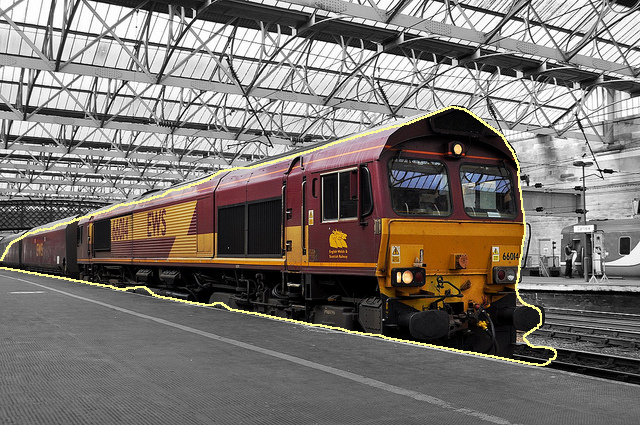
\includegraphics[scale=0.16]{figures/coco/completion/train/corrected-seg-with-data.png}
}%
\caption{\textbf{Contour completion.} The GF model favors connected components due to the completion effect of the elastica energy. That is particularly useful to avoid oversegmentation.}
\label{fig:coco-completion}
\end{figure}

\begin{figure}
\center
\subfloat[$34$ iterations ($63$s).]{
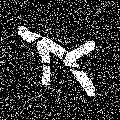
\includegraphics[scale=0.5]{figures/chan-vese-alike/branch/branch-noisy.png}
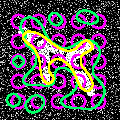
\includegraphics[scale=0.5]{figures/chan-vese-alike/branch/contours.png}
}\hspace{1em}%
\subfloat[$35$ iterations ($53$s).]{
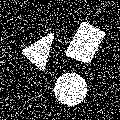
\includegraphics[scale=0.5]{figures/chan-vese-alike/simple-geometry/simple-geometry-noisy.png}
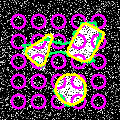
\includegraphics[scale=0.5]{figures/chan-vese-alike/simple-geometry/contours.png}
}%
\caption{\textbf{Chan-Vese alike data term.} The initial contour is highlighted in pink and the final contour in yellow. An intermediate contour is also highlighted in green. A proper parameter setting favors component completion (left) or component break (right). Images are $100\times100$. }
\label{fig:GF-chan-vese-alike}
\end{figure}



\section{Conclusion}

We presented a discrete shape evolution algorithm driven by the elastica energy. The GF model is built on recent results on the multigrid convergence of curvature and tangent estimators and its main step consists in to compute the minimum cut of candidate graphs. A candidate graph is constructed for each element in a neighborhood of shapes of the current digital set and its minimum cut gives a candidate shape. At each iteration, the GF model selects the candidate shape with lowest elastica energy. We have shown that our model can escape local minimum in the shape evolution problem by using a very simple neighborhood scheme of shapes. Indeed, our experiments converged to the shape of minimum elastica energy. 

Next, we presented some applications in image processing tasks. The GF model delivery contour with lower inflection points, smooth tangent profile and lower elastica energy than those by grabcut. That is done while keeping high values of precision and recall with respect the Coco annotated images used in our experiments. Finally, we presented an unsupervised segmentation model based on the classical Chan-Vese data term, which demonstrate the flexibility of the model. 

One of the strengths of our model is that the curvature estimation is based on digital data only and it is not attached to a curve model, which may restrict the curve evolution and pose problems in its update. Secondly, the GF model is highly parallelizable. We believe that a GPU implementation will greatly reduce the running times of our algorithm for all the presented applications. The bottleneck is in the minimum cut computation, as it is difficult to come up with a parallel implementation, but since the latter is computed along a thin band of the shape contour, we believe that this is a minor problem.

There are some possible paths for future work. Firstly, the graph construction part of the algorithm can be optimized. In the current version, the graph is constructed at every iteration, but most of the time, the graph structure changes very slightly and this can be used to optimize its construction. Secondly, we use a very rough neighborhood of shapes that dilates or erodes the initial shape. The contour completion property of the model can be better exploited by employing different neighborhoods. For example, we could alongate the initial shapes in regions of high curvature to obtain a stretched neighborhood of shapes. This could be particularly useful in the segmentation of thin and elongated objects as blood vessels.


\bibliographystyle{alpha}
\bibliography{gf-paper}

\end{document}

